\documentclass[12pt,diff_rus]{article} % for LaTeX 2e
\usepackage[utf8]{inputenc}        % LaTeX distr. specific
\usepackage[colorlinks=false]{hyperref}
\usepackage[english,russian]{babel} % LaTeX distr. specific
\usepackage{amssymb,amscd,amsmath}    % стиль AMS и русские переносы
\usepackage{diff_rus}                  % стиль для колонтитулов журнала

\usepackage{graphicx} % Required for inserting images

%\usepackage[russian, english]{babel}
\usepackage{MnSymbol}
\usepackage[active]{srcltx}
\usepackage[final]{pdfpages}

\usepackage{wrapfig}
\usepackage{amsmath}
\usepackage{MnSymbol}
\usepackage{wasysym}

\usepackage{tikz}
\usepackage{subfig}
\usepackage{listings}
\usepackage{bigints}
\usepackage{changepage}

\usepackage[labelsep=period]{caption}
\usetikzlibrary{arrows,decorations.pathmorphing,backgrounds,positioning,fit,petri}
\usepgflibrary{arrows} % LATEX and plain TEX and pure pgf
\usetikzlibrary{arrows} % LATEX and plain TEX when using Tik Z
\definecolor{whitesmoke}{rgb}{0.9,0.9,0.9} \definecolor{whitesmoke2}{rgb}{0.8,0.8,0.8}

\def\e{\varepsilon}
\newcommand{\pp}{\varphi}
\catcode`@=11
\def\caseswithdelim#1#2{\left#1\,\vcenter{\normalbaselines\m@th
  \ialign{\strut$##\hfil$&\quad##\hfil\crcr#2\crcr}}\right.}% you might like it without the \strut
\catcode`@=12
%
\def\bcases#1{\caseswithdelim[{#1}}
\def\vcases#1{\caseswithdelim|{#1}}
%
% Пакеты по желанию (самые распространенные)
% Хитрые мат. символы
\usepackage{euscript}
% Таблицы
\usepackage{longtable}
\usepackage{makecell}

\setlength{\textwidth}{170mm}          % ширина текста
\setlength{\textheight}{240mm}         % высота текста (без учета колонтитула)
\setlength{\topmargin}{-20mm }         % расстояние от верхнего обреза листа
\setlength{\evensidemargin}{0mm}       % до колонтитула
\setlength{\oddsidemargin}{0mm}        % до колонтитула = 1 дюйм + значение
                                       % параметра
\setlength{\parskip}{4pt}              % абзацный пропуск
\setlength{\parindent}{2em}            % абзацный отступ
\setlength{\arrayrulewidth}{0.8pt}     % толщина линий разграфки
\setlength{\doublerulesep}{6pt}        % ширина пробела между соседними
                                       % параллельными линиями таблицы
\renewcommand{\arraystretch}{1.15}     % коэффициент увеличения межстрочного
                                       % интервала в таблице

\tolerance=10000
\hbadness=10000
\vbadness=10000

%%%%%%%%%%%%%%%%%%%%%%%%%%%%%%%%%%%%%%%%%%%%%%%%%%%%%%%%%%%%%%%
%%%
%%% Внесите исправления в файлы DIFF_RUS.TEX и DIFF_RUS.STY
%%%
%%%%%%%%%%%%%%%%%%%%%%%%%%%%%%%%%%%%%%%%%%%%%%%%%%%%%%%%%%%%%%%


%%%%%%%%%%%%%%%%%%%%%%%%%%%%%%%%%%%%%%%%%%%%%%%%%%%%%%%%%%%%%%%
%%% Выставите номер страницы
\setcounter{page}{1}                   % номер первой страницы
%%%%%%%%%%%%%%%%%%%%%%%%%%%%%%%%%%%%%%%%%%%%%%%%%%%%%%%%%%%%%%%
\renewcommand{\refname}{Литература}
\newtheorem{definition}{Определение}
\newtheorem{theorem}{Теорема}
\newtheorem{proposition}{Утверждение}
\newtheorem{corollary}{Следствие}


\begin{document}
\input{diff_rus.tex}

%%%%%%%%%%%%%%%%%%%%%%%%%%%%%%%%%%%%%%%%%%%%%%%%%%%%%%%%%%%%%%%
%%% Имя файла Вашей статьи
В работе рассматривается двумерная автономная система дифференциальных уравнений:

\begin{equation}
\begin{cases}
      \dot x=-xy^2+x+y,\\
      \dot y=-x-y+x^2y.
    \end{cases}
    \label{eq:first}
\end{equation}

Для системы (\ref{eq:first}) был найден первый интеграл (см. \cite{basov}, \cite{engl}), но общее решение найдено не было. Для нахождения общего решения был использован метод, который основывается на построении периодической функции, опираясь на обратную функцию к неберущемуся интегралу. Такой подход к решению систем дифференциальных уравнений представляет не только теоретический интерес, но также может иметь практическое применение в различных областях, где возникают аналогичные задачи.\\

Рассматриваемый пример можно использовать для решения задач, связанных с 16-ой проблемой Гильберта, а точнее, локальной проблемой Арнольда-Гильберта. Для этого правую часть системы (\ref{eq:first}) следует рассматривать как невозмущенную часть системы, зависящей от малого автономного или периодического возмущения с последующим исследованием числа сохранившихся предельных циклов в случае автономного возмущения или инвариантых торов в случае периодического.\\

\medskip 
Рассмотрим систему (\ref{eq:first}):

$$
\begin{cases}
      \dot x=-xy^2+x+y,\\
      \dot y=-x-y+x^2y.
    \end{cases}
$$

Составим интегрируемую комбинацию.

\smallskip
Реализуя общую идею убирать в правых частях какие-то слагаемые, можно избавиться от $x$ в первом уравнении и от $-y$  
во втором. Попробовать это сделать имеет смысл, так как в левой части возникнет формула производной произведения. Имеем:

\smallskip
$y\dot x+x\dot y=y^2-xy^3-x^2+x^3y\ \Leftrightarrow\ \dot{(xy)}=(x^2-y^2)(xy-1).$

\smallskip
Само по себе это уравнение ничего пока не дало, так как в правой части помимо произведения есть еще разность квадратов. 
Поэтому избавимся в правой части системы от кубических слагаемых тем более, что слева появляется производная суммы квадратов. Имеем: 

\smallskip
\begin{equation}
    \dot x^2+\dot y^2=2(x^2-y^2).\label{eq:second}
\end{equation}

\smallskip
Подставляя отсюда $x^2-y^2$ в первое уравнение, получаем интегрируемую комбинацию $\dot{(xy)}=(\dot x^2+\dot y^2)(xy-1)/2.$\\

Следовательно, $xy=1$ или 
\smallskip
$2(xy-1)^{-1}d(xy)=d(x^2+y^2)$.\\

Интегрируя, получаем $ 2\ln|xy-1|-x^2-y^2=C$ --- первый интеграл системы, который удобно записать в виде:
\smallskip\noindent
\begin{equation}
    xy - 1 =C e^{(x^2+y^2)/2}, 
\label{eq:third}
\end{equation}

\noindent поскольку в (\ref{eq:third}) входит решение $xy = 1$.

Подставляя $xy=1$ в первое уравнение системы (\ref{eq:first}) получаем уравнение $\dot x=x,$ из которого находим однопараметрическое семейство решений $$x(t)=Ce^{t},\ y(t)=C^{-1}e^{-t}.$$

К сожалению, еще один первый интеграл, а с ним вместе и общее решение системы, найти при помощи создания интегрируемой комбинации не удается. Поэтому будем искать общее решение другим способом.\\

Решая систему $-xy^2+x+y = 0$ и $-x-y+x^2y = 0$,
 находим три особые точки системы (\ref{eq:first}) : $(0,0),$ $ (\sqrt{2}, \sqrt{2})$, $ (-\sqrt{2}, -\sqrt{2})$. \\

Чтобы найти ограничения на константу $C$ в (\ref{eq:third}), исследуем функцию 
\begin{equation}
            C(x,y) = (xy-1)e^{-(x^2+y^2)/2},
    \label{eq:seventh}
\end{equation}
\noindent причем $C(0,0) = 1, C(\sqrt{2},\sqrt{2}) = C(-\sqrt{2}, -\sqrt{2}) = e^{-2}.$\\

Градиент функции (\ref{eq:seventh}) $\nabla C(x,y) = \left (\cfrac{\partial C}{\partial x}, \cfrac{\partial C}{\partial y} \right)$ имеет вид:\\$ \nabla C(x,y) = (e^{-(x^2+y^2)/2}(-x^2y + x + y),$ $ e^{-(x^2+y^2)/2}(-y^2x + x + y))$.\\

Следовательно, $\nabla C(x,y)=0$ только в особых точках.\\

Рассмотрим замкнутую окрестность $\overline{V}_2(O) = \{(x,y): x^2 + y^2 \leq 4\}$ начала координат O = $(0,0)$. Поскольку все особые точки принадлежат этому компакту, для нахождения максимального и минимального значений функции (\ref{eq:seventh}) на $\overline{V}_2(O)$ достаточно сравнить значения функции в особых точках (\ref{eq:seventh}) с ее значениями на границе $\partial \overline{V}_2(O) = \{(x,y): x^2 + y^2 = 4\}$. Для этого в (\ref{eq:seventh}) удобно перейти к полярным координатам:\smallskip
\begin{equation}
     \begin{cases}
         x = r \cos{\theta},\cr
         y = r \sin{\theta},
     \end{cases}
     \label{eq:eight}
\end{equation}
получая функцию $C(r, \theta) = \Bigg(\cfrac{1}{2}\,r^2\sin{2\theta} - 1\Bigg)e^{-r^2/2}$.\\

Заметим, что:
\begin{equation}
  C_*(r) = \Bigg(-\cfrac{1}{2}\,r^2 - 1\Bigg)e^{-r^2/2} \leq C(r, \theta) \leq C^*(r) = \Bigg(\cfrac{1}{2}\,r^2 - 1\Bigg)e^{-r^2/2}. 
  \label{eq:ninth}
\end{equation}

Пусть $r \geq 2$. Тогда $C_*(r) > 0$, $C_*(r) ' > 0$ и $C_* (2) = -3e^{-2} \leq C_* (r) < 0$. Аналогично, $C^*(r) > 0$, $C^*(r) ' \leq 0$ и $0<C^* (r)\leq C^* (2) = e^{-2} $. Отсюда следует:
$$-3e^{-2} \leq C_* (r) < C(x,y) = C(r, \theta)<C^* (r) \leq e^{-2}.$$

\begin{figure}[ht!]%
    \begin{center}
    {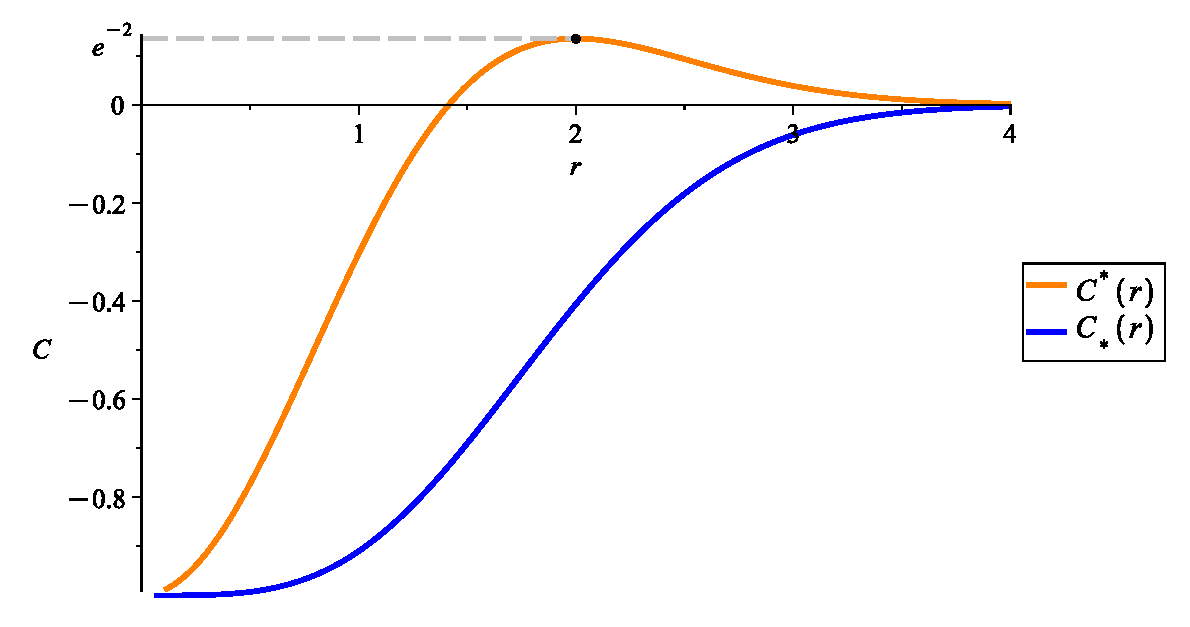
\includegraphics[scale=0.7]{mmrcd2.eps} }%
    \caption{Графики $C_*(r)$ и $C^*(r)$}%
    \label{fig:first}
    \end{center}%
\end{figure}

Таким образом, для всех $(x,y) \in \overline{V}_2(O) $ верно, что $-1 \leq C(x,y)\leq e^{-2}$.

Пусть теперь $(x, y) \in \mathbb{R}^2\,\, \backslash\,\, \overline{V}_2(O)$. Поскольку 2 < $r = \sqrt{x^2 + y^2}$, то $-1 \leq -3e^{-2} < C(r,\theta) = C(x,y) \leq e^{-2}$, т.е. для всех точек $(x,y)$ верно неравенство $-1 < C(x,y)\leq e^{-2}$.\\

В результате, $C(x,y) \in [-1, e^{-2}]$ для всех $(x,y)\in \mathbb{R}^2$.\\

Исследуем линии уровня первого интеграла (\ref{eq:third}):
\begin{enumerate}
\item[{1)}] при $C = -1$ имеем особую точку (0, 0) ;
\item[{2)}] для любого $C \in (-1, 0)$ имеем цикл расположенный в области $xy<1$;
\item[{3)}] при $C = 0$ имеем гиперболу $xy = 1$, объединяющую две траектории: $y = x^{-1}$ при $x > 0$ и $y = x^{-1}$ при $x < 0$;
\item[{4)}] для любого $C \in (0, e^{-2})$ имеем два симметричных цикла: первый в области $xy>1$ и $x< 0$, второй в области $xy>1$ и $x> 0$, охватывающие особые точки $(-\sqrt{2}, -\sqrt{2})$ и $(\sqrt{2}, \sqrt{2})$ соответственно.
\item[{5)}] при $C = e^{-2}$ имеем особые точки $(\sqrt{2}, \sqrt{2})$, $(-\sqrt{2}, -\sqrt{2})$.
\end{enumerate}

\begin{figure}[ht!]%
    \begin{center}
    {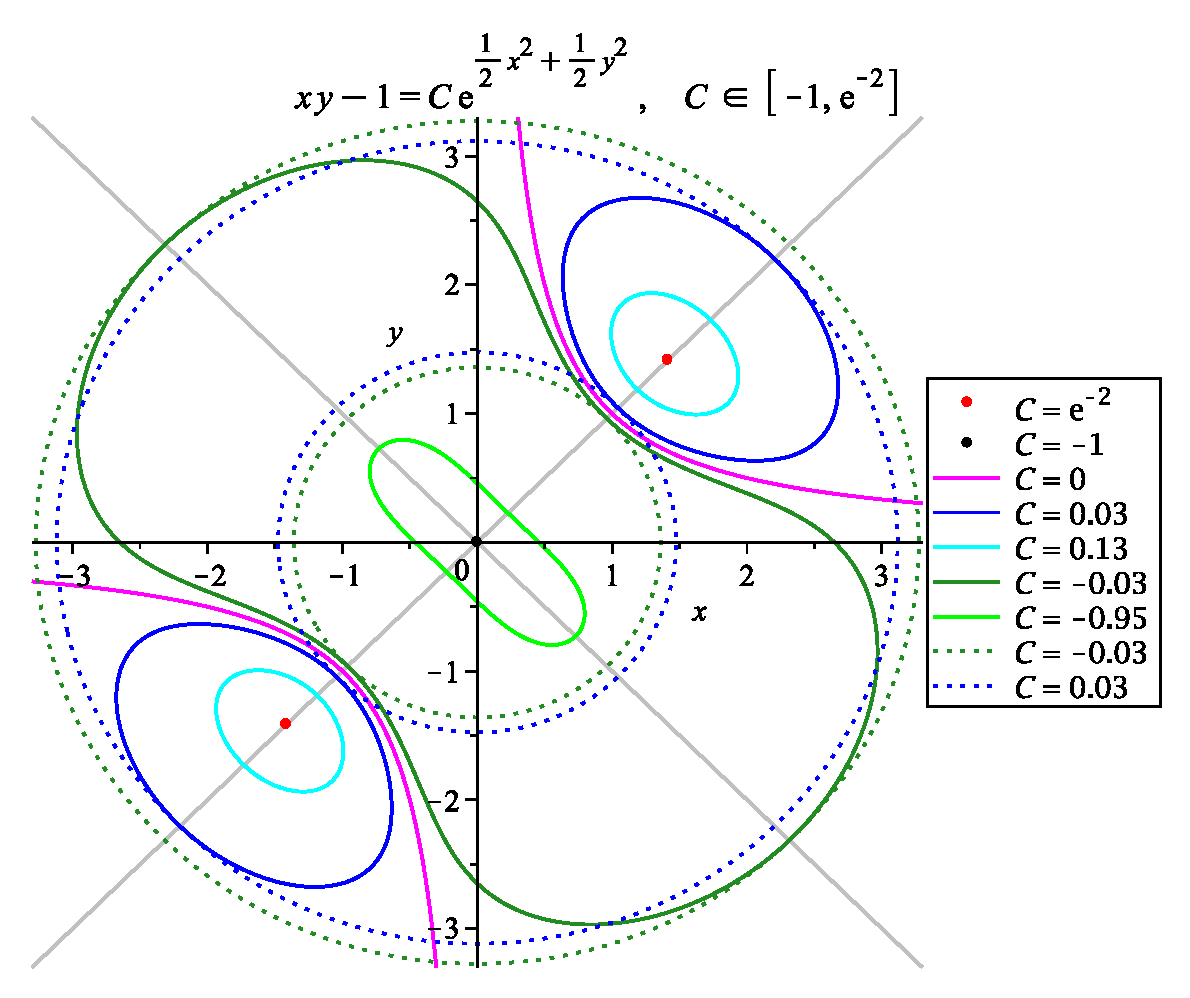
\includegraphics[scale=0.65]{zik.eps} }%
    \caption{Фазовый портрет системы (1)}%
    \label{fig:second}
    \end{center}%
\end{figure}

Первый интеграл (\ref{eq:third}) после полярной замены (\ref{eq:eight}) примет вид: \begin{equation}
     2^{-1}r^2\sin(2\theta) - 1 = Ce^{r^2/2} \hbox{, или }  \sin(2\theta) = 2r^{-2}(Ce^{r^2/2}+1), \label{eq:forth}
 \end{equation}
 
\noindent а уравнение (\ref{eq:second}) сведётся к уравнению \begin{equation}
     \dot{r}^2 = 2r^2\cos(2\theta)\hbox{, или }\dot r = r\cos(2\theta). \label{eq:fivth}
 \end{equation}

Поскольку $\cos(2\theta) = \pm \sqrt{1-\sin^2(2\theta)}$, то после подстановки (\ref{eq:forth}) в (\ref{eq:fivth}) для вяского $C \in [-1; e^{-1}]$ получаем уравнения с разделяющимися переменными:
\begin{equation}
    \dot r = \pm \sqrt{r^2 - 4r^{-2}(Ce^{r^2/2}+1)^2}.\label{eq:sixth}
\end{equation}

Найдем область определения $D$ функции 
$$f(r, C) = (r^2 - 4r^{-2}(Ce^{r^2/2}+1)^2)^{-1/2}.$$

Из неравенств $r^2 - 4r^{-2}(Ce^{r^2/2}+1)^2) > 0$ и $r > 0$ вытекает, что $r^2 > 2|C e^{r^2/2} + 1|$.\\

Таким образом, $D$ --- это область заключенная между двумя кривыми, которые задаются функциями из (\ref{eq:ninth}): $C^*(r)$ и $C_*(r)$ (см. рис. \ref{fig:first}).\\

Найдем область определения функции $f(r, C)$ по переменной $r$ при финсированной константе $C$.\\

Функция $C_*(r)$ строго монотонно возрастает при $r>0$, поэтому существует обратная функция ${(C_*)}^{-1}(C)$ при $C\in(-1, 0)$.\\

Функция $C^*(r)$ строго монотонно возрастает при $r\in(0, 2)$ и строго монотонно убывает при $r>2$.\\

Положим $C_{+}^*(r) = C^*(r)$ при $r\in(0, 2)$ и  $C_{-}^*(r) = C^*(r)$ при $r>0$. Тогда существуют обратные функции ${(C_{+}^*)}^{-1}(C)$ при $ C\in(-1, e^{-2})$ и ${(C_{-}^*)}^{-1}(C)$ при $C\in(0, e^{-2})$. Пусть:

\begin{equation*}
r_*(C) = {(C_{+}^*)}^{-1}(C)\hbox{ при } C\in(-1, e^{-2}),\,\,\,\,
 r^*(C) =
\bcases{
{(C_*)}^{-1}(C)\hbox{ при } C\in(-1, 0),\cr
{(C_{-}^*)}^{-1}(C)\hbox{ при } C\in(0, e^{-2}).
}
\end{equation*}


Таким образом, функция $f(r,C)$ определена для любого $r\in(r_*(C), r^*(C))$.\\

\begin{figure}[ht!]
\begin{center}
    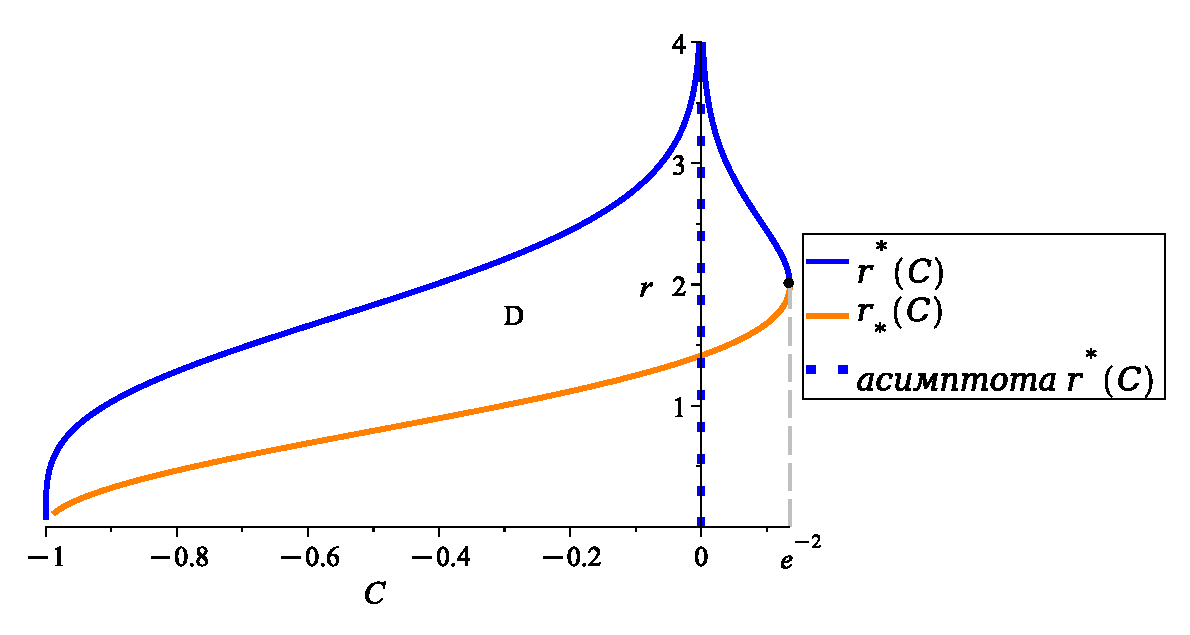
\includegraphics[scale=0.6]{mmrc.eps}
\caption{Графики $r_*(C)$ и $r^*(C)$}
\label{fig:third}
\end{center}
\end{figure}

Случаи когда константа $C$ равна $0$, $-1$ или $e^{-2}$ тривиальны и в дальнейшем рассматриваться не будут (см. рис. \ref{fig:second}).\\

Для всякого $C \in (-1; e^{-1}) \backslash 0$ и $r, r_0 \in (r_*(C), r^*(C))$ положим:
$$
F_+(r, r_0, C) = \int_{r_{0}}^r f(\xi, C)d\xi,\, F_-(r, r_0, C) = - F_+(r, r_0, C). 
$$

Заметим, что функция $F_+(r, r_0, C)$ строго монотонно возрастает по $r$, так как $f(r,C) >0$.\\Аналогично, $F_-(r, r_0, C)$ строго монотонно убывает по r.


Тогда для любого $C\in (-1; e^{-1}) \backslash 0$ общими решениями уравнений (\ref{eq:sixth}) будут функции:
$$
\displaylines{
\bcases{
    t(r, r_0,C) = F_+(r,r_0,C) \cr
    t(r,r_0,C) = F_-(r,r_0,C)\cr
}}
$$

Введем обратные функции:
$$r_+(t, r_0,C) = {F_+}^{-1}(t,r_0,C)\hbox{, } r_-(t,r_0,C) = {F_-}^{-1}(t,r_0,C).$$

Проведем анализ поведения радиус-вектора на фазовых траекториях системы (\ref{eq:first}). Рассмотрим два случая:
\begin{enumerate}
    \item [{1)}] пусть $C\in(0, e^{-2})$. Для определенности возьмем цикл в области $xy > 1$ и $x > 0$. Тогда после замены координат в уравнении (\ref{eq:third}) на $x = y = r\cos{\pi/4}$ получим $r = \sqrt{2C e^{r^2/2} + 2}$, что есть уравнение, которое задает $r_*(C)$ и $r^*(C)$, т.е. максимум и минимум радиуса решения, которое движется по заданной траектории достигаются в точках пересечения уравнения (\ref{eq:third}) и прямой $y = x$ (см. рис. \ref{fig:second}). Аналогично для цикла в области $xy > 1$ и $x < 0$;
    \item [{2)}] при $C\in(-1, 0)$ будем рассматривать две замены: $x = y = r\cos{\pi/4}$, и $x = r\cos{3\pi/4}$, $y = -r\cos{3\pi/4}$. Следовательно, минимум радиуса достигается в точках пересечения уравнения (\ref{eq:third}) и прямой $y = x$, а максимум в точках пересечения уравнения (\ref{eq:third}) и прямой $y = -x$ (см. рис. \ref{fig:second}). 
\end{enumerate}

\textbf{Утверждение}.\textit{ Несобственный интеграл $F_+(r^*(C), r_0,C)$ сходится.}\\ 
Д\,о\,к\,а\,з\,а\,т\,е\,л\,ь\,с\,т\,в\,о. От противного. Предположим, что $F_+(r^*(C), r_0, C)$ расходится, т.е. точка максимума не достигается за конечное время. Следовательно, не существует периодического решения. С другой стороны, поскольку решение определено на всей оси времени(см. \cite{basov}) и находится на замкнутой кривой, то имеем периодическое решение. Противоречие.\\
Аналогично для $F_-(r_*(C), r_0, C)$.\\

Таким образом, функции $F_\pm(r,r_0, C)$ существуют и конечны для $r \in [r_*(C), r^*(C)]$, $r_0 \in [r_*(C), r^*(C)]$.

\begin{figure}[ht!]
\begin{center}
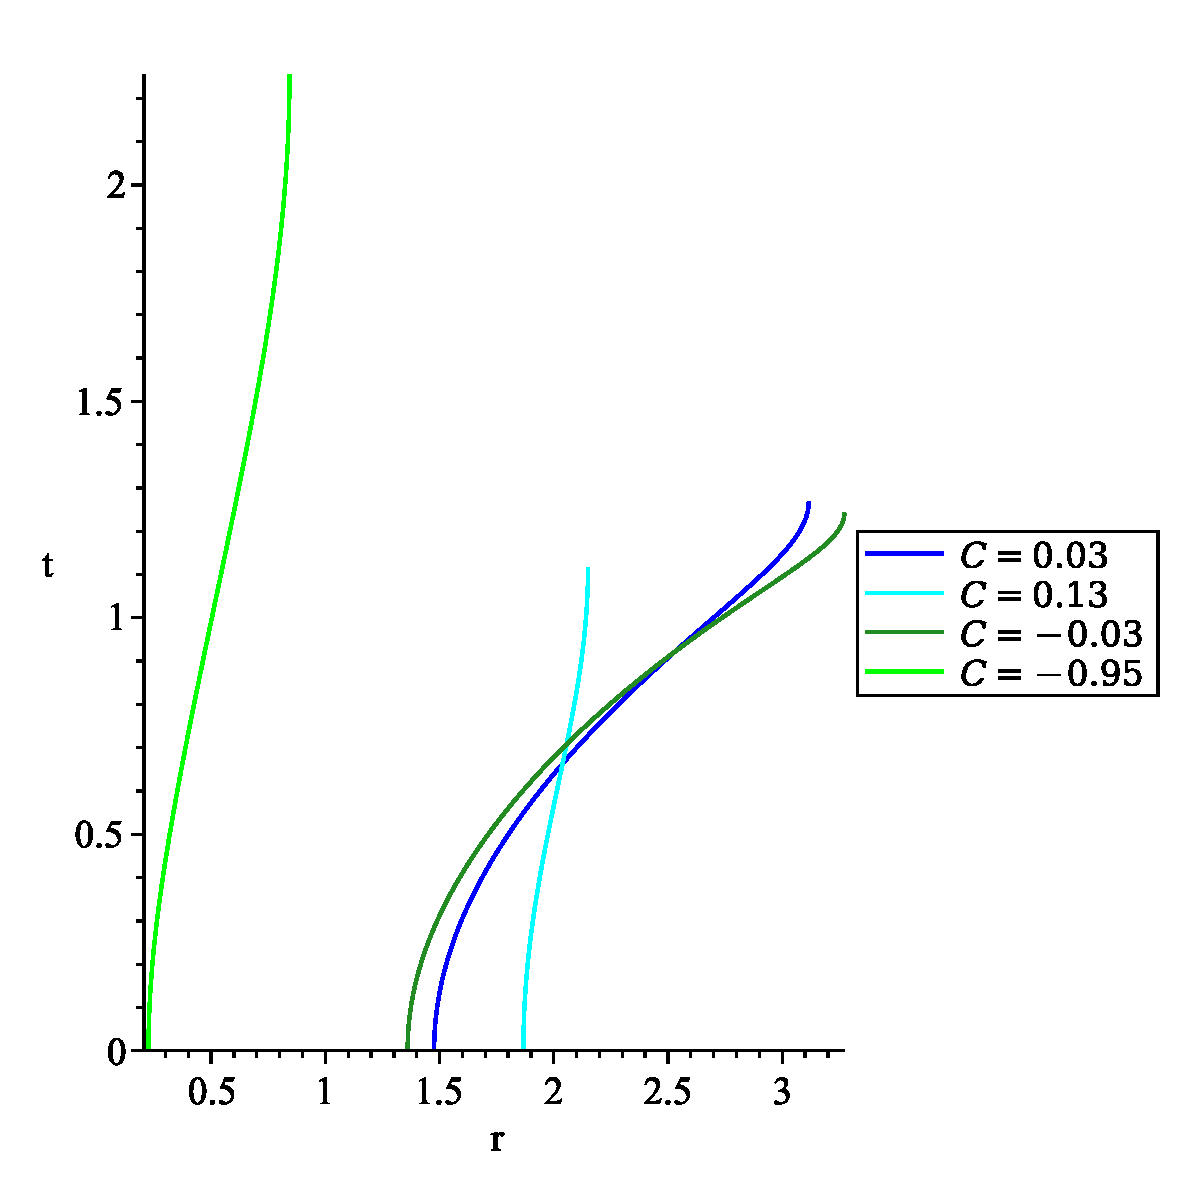
\includegraphics[scale=0.48]{Frad.eps}
\caption{Графики $F_+(r, r_*(C), C)$}
\end{center}
\end{figure}

Пусть $\omega(C) = F_+(r^*(C),r_*(C), C)$. Тогда при $C < 0$ период решения $\Omega(C)$ = $ 2F_+(r^*(C),r_*(C), C) + 2F_-(r_*(C), r^*(C), C) = 4\omega(C)$,\\ если $C > 0$, то $\Omega(C) = F_+(r^*(C),r_*(C), C) + F_-(r_*(C), r^*(C), C) = 2\omega(C)$.
\begin{figure}[ht!]
\begin{center}
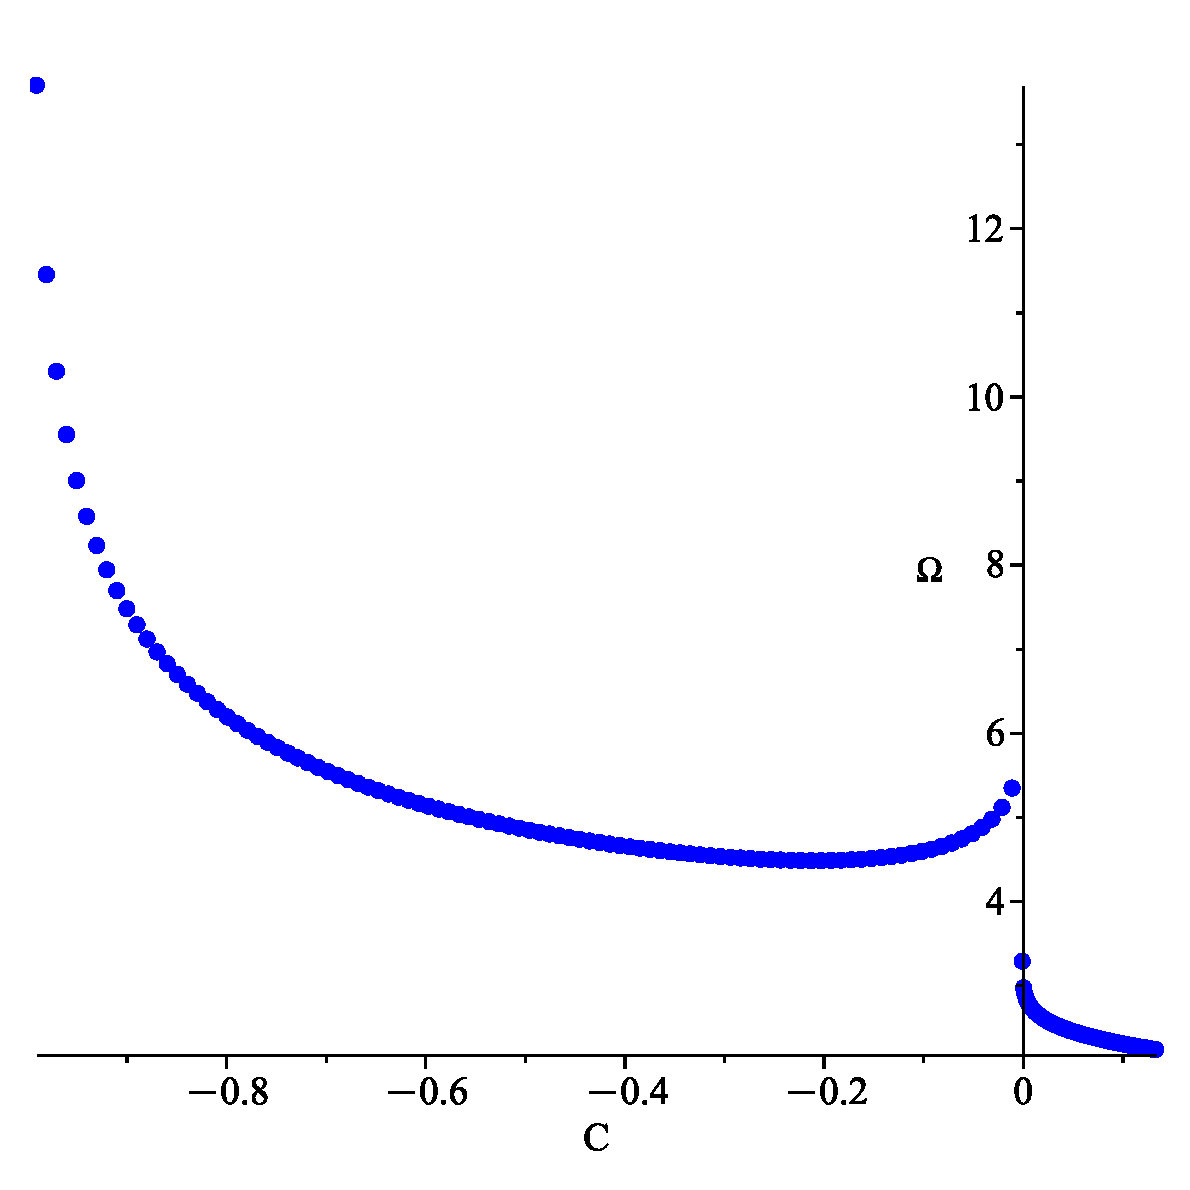
\includegraphics[scale=0.45]{omega.eps}
\caption{График $\Omega(C)$}
\end{center}
\end{figure}
\newpage
Построим периодическое решение $R(t,r_0, C)$ из функций $r_+(t, r_0, C)$ и $r_-(t,r_0, C)$ на всем промежутке времени. Известно, что $r_+(t,r_0, C)$ монотонно возрастает в зависимости от t, а $r_-(t,r_0,C)$ монотонно убывает. Рассмотрим два случая:
\begin{enumerate}
    \item[{1)}] пусть $\dot r < 0$, т.е. радиус убывает. Тогда время за которое точка дойдёт до минимума радиуса $\tau^-(r_0, C)$ =  $F_-(r_*(C), r_0, C)$. Имеем:
    \begin{gather*}
        R_-(t,t_0, r_0, C) =\\
        \bcases{
        r_+(t-2\tau^-(r_0,C) -2k\omega(C)-t_0, r_*(C),C),\cr \hspace{15pt} t\in(2k\omega(C)+\tau^-(r_0,C)+t_0;(2k+1)\omega(C)+\tau^-(r_0,C)+t_0],\cr
        r_-(t-2k\omega(C)- t_0, r^*(C),C),\cr \hspace{15pt} t\in((2k-1)\omega(C)+\tau^-(r_0,C) + t_0;2k\omega(C)+\tau^-(r_0,C)+t_0],
    }\\
    \forall k \in \mathbb{Z};
\end{gather*}
   
    \item[{2)}] при $\dot r > 0$ радиус будет возрастать. Пусть время за которое точка дойдёт до максимума радиуса $\tau^+(r_0,C)$ =  $F_+(r^*(C), r_0, C)$. Тогда:
    \begin{gather*}
    R_+(t,t_0, r_0, C) =\\
    \bcases{
        r_+(t-2k\omega(C)-t_0, r_*(C),C),\cr \hspace{15pt} t\in((2k-1)\omega(C)+\tau^+(r_0,C)+t_0;2k\omega(C)+\tau^+(r_0,C)+t_0],\cr
        r_-(t-2\tau^+(r_0,C)-2k\omega(C)-\omega(C)-t_0, r^*(C),C),\cr \hspace{15pt} t\in(2k\omega(C)+\tau^+(r_0,C)+t_0;(2k+1)\omega(C)+\tau^+(r_0,C)+t_0],
    } \\
    \forall k \in \mathbb{Z}.
    \end{gather*}
\end{enumerate}

\begin{figure}[ht!]
\begin{center}
    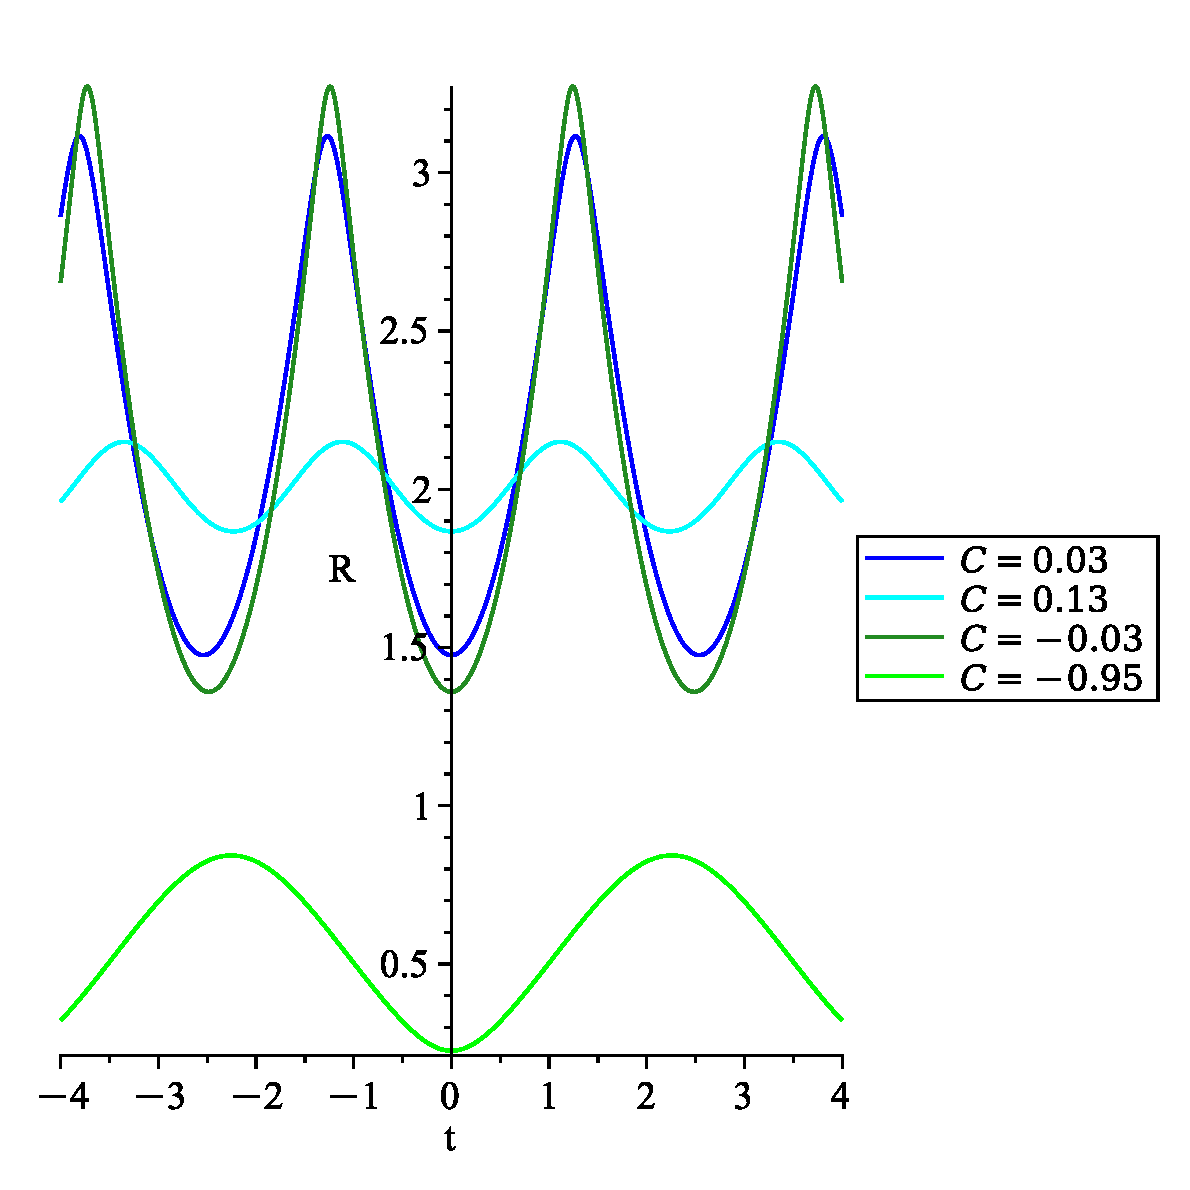
\includegraphics[scale=0.48]{Radfull.eps}
\caption{Графики $R_+(t, 0, r_*(C), C)$}
\end{center}
\end{figure}

Рассмотрим зависимость производной радиуса от угла в равенстве (\ref{eq:fivth}). Тогда $\dot{r} < 0 \Leftrightarrow \cos{2\theta} <0$ и $\dot{r} > 0 \Leftrightarrow \cos{2\theta} >0$. Имеем:
$$
\dot{r} < 0 \Leftrightarrow -\cfrac{\pi}{4} + \pi n < \theta < \cfrac{\pi}{4} + \pi n , n\in \mathbb{Z} \hbox{ и }$$
$$
\dot{r} > 0 \Leftrightarrow \cfrac{\pi}{4} + \pi m < \theta < \cfrac{3\pi}{4} + \pi m, m\in \mathbb{Z}.
$$

\begin{figure}[ht!]%
    \begin{center}
    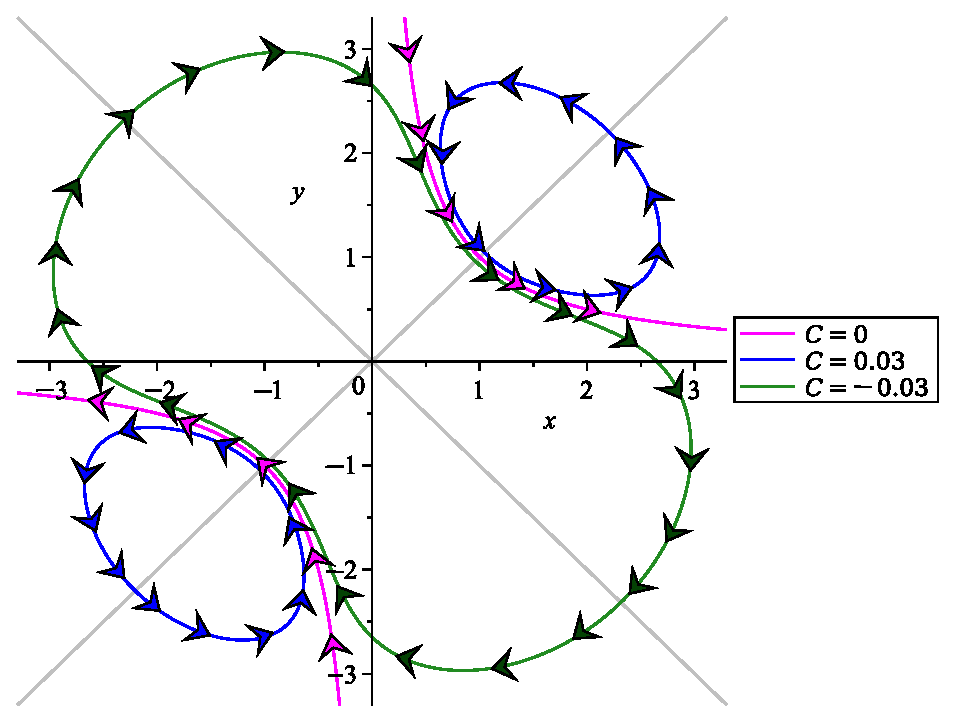
\includegraphics[scale = 0.48]{divdiff.eps}
    \caption{Направление движения на кривых}%
    \label{fig:seventh}
    \end{center}%
\end{figure}

Вернемся к уравнению (\ref{eq:forth}). Пусть $h(r,C) = 2r^{-2}(Ce^{r^2/2}+1)$.\\
Рассмотрим два случая:
\begin{enumerate}
    \item[{1)}] при $C > 0$ возьмём для определённости цикл в области $x y > 1$ и $x > 0$. Из уравнения (\ref{eq:forth}) имеем: $\theta(r,C) $= $\cfrac{(-1)^k }{2}\,\arcsin{h(r,C)}$+$\cfrac{\pi}{2}\,k$. Более того, в данной области угол $\theta \in (0, \pi/2)$. Следовательно, $\theta_+(r,C) =\cfrac{1}{2}\, \arcsin{h(r,C)}$, или $\theta_-(r,C) =-\cfrac{1}{2}\arcsin{h(r,C)}$+$\cfrac{\pi}{2}$. Заметим, что $\theta_-(r,C)$ показывает изменение угла для верхней половины траектории, где $\dot{r} > 0$, а $\theta_+(r,C)$ - для нижней, где $\dot {r} < 0$. Для случая, когда радиус начальной точки убывает имеем:
     \begin{gather*}
     \Theta^+_-(t,t_0,r_0,C) =\\
     \bcases{\theta_+(R_-(t,t_0,r_0,C),C)
    ,\cr\hspace{35pt} t\in(2k\omega(C)+\tau^-(r_0, C)+t_0;(2k+1)\omega(C)+\tau^-(r_0, C)+t_0],\cr
    \theta_-(R_-(t,t_0,r_0,C),C),\cr\hspace{35pt} t\in((2k-1)\omega(C)+\tau^-(r_0, C) + t_0;2k\omega(C)+\tau^-(r_0, C)+t_0],
    }\\
     \forall k \in \mathbb{Z},
    \end{gather*}
    
    если радиус возрастает имеем:
    \begin{gather*}
     \Theta^+_+(t,t_0,r_0,C) =\\
     \bcases{\theta_+(R_+(t,t_0,r_0,C),C)
    ,\cr\hspace{40pt} t\in((2k-1)\omega(C)+\tau^+(r_0, C)+t_0;2k\omega(C)+\tau^+(r_0, C)+t_0],\cr
    \theta_-(R_+(t,t_0,r_0,C),C),\cr\hspace{40pt} t\in(2k\omega(C)+\tau^+(r_0, C)+t_0;(2k+1)\omega(C)+\tau^+(r_0, C)+t_0],
    }\\
     \forall k \in \mathbb{Z};
    \end{gather*}
   
\item[{2)}] при $C < 0$ функция $h(r,C)$ монотонно убывает и неограничена. Следовательно, угол $\theta\in [-\pi/4, 7\pi/4)$. Рассмотрим случай при угле начальной точки $\theta_0 \in [-\pi/4; 3\pi/4]$. Поскольку имеем периодическое решение с периодом 4$\omega$, то, если радиус начальной точки убывает, получаем:

 \begin{gather*}
     \Theta^-_-(t,t_0,r_0,C) =\\
     \bcases{
     \theta_+(R_-(t,t_0,r_0,C),C)
    ,\cr\hspace{20pt} t\in(4k\omega(C)+\tau^-(r_0, C)+t_0;(4k+1)\omega(C)+\tau^-(r_0, C)+t_0],\cr
    \theta_-(R_-(t,t_0,r_0,C),C) + \pi,\cr\hspace{20pt} t\in((4k-1)\omega(C)+\tau^-(r_0, C) + t_0;4k\omega(C)+\tau^-(r_0, C)+t_0],\cr
    \theta_+(R_-(t,t_0,r_0,C),C)+\pi
    ,\cr\hspace{20pt} t\in((4k-2)\omega(C)+\tau^-(r_0, C)+t_0;(4k-1)\omega(C)+\tau^-(r_0, C)+t_0],\cr
    \theta_-(R_-(t,t_0,r_0,C),C),\cr\hspace{20pt} t\in((4k-3)\omega(C)+\tau^-(r_0, C) + t_0;(4k-2)\omega(C)+\tau^-(r_0, C)+t_0],
    }\\
    \forall k \in \mathbb{Z},
 \end{gather*}
    
если начальный радиус возрастает получаем:

 \begin{gather*}
 \Theta^-_+(t,t_0,r_0,C) =\\
     \bcases{
     \theta_+(R_+(t,t_0,r_0,C),C)
    ,\cr\hspace{20pt} t\in(4k\omega(C)+\tau^-(r_0, C)+t_0;(4k+1)\omega(C)+\tau^-(r_0, C)+t_0],\cr
    \theta_-(R_+(t,t_0,r_0,C),C) + \pi,\cr\hspace{20pt} t\in((4k-1)\omega(C)+\tau^-(r_0, C) + t_0;4k\omega(C)+\tau^-(r_0, C)+t_0],\cr
    \theta_+(R_+(t,t_0,r_0,C),C)+\pi
    ,\cr\hspace{20pt} t\in((4k-2)\omega(C)+\tau^-(r_0, C)+t_0;(4k-1)\omega(C)+\tau^-(r_0, C)+t_0],\cr
    \theta_-(R_+(t,t_0,r_0,c),C),\cr\hspace{20pt} t\in((4k-3)\omega(C)+\tau^-(r_0, C) + t_0;(4k-2)\omega(C)+\tau^-(r_0, C)+t_0],
    }\\
     \forall k \in \mathbb{Z}.
 \end{gather*}

\end{enumerate}

\begin{figure}[ht!]%
    \begin{center}
    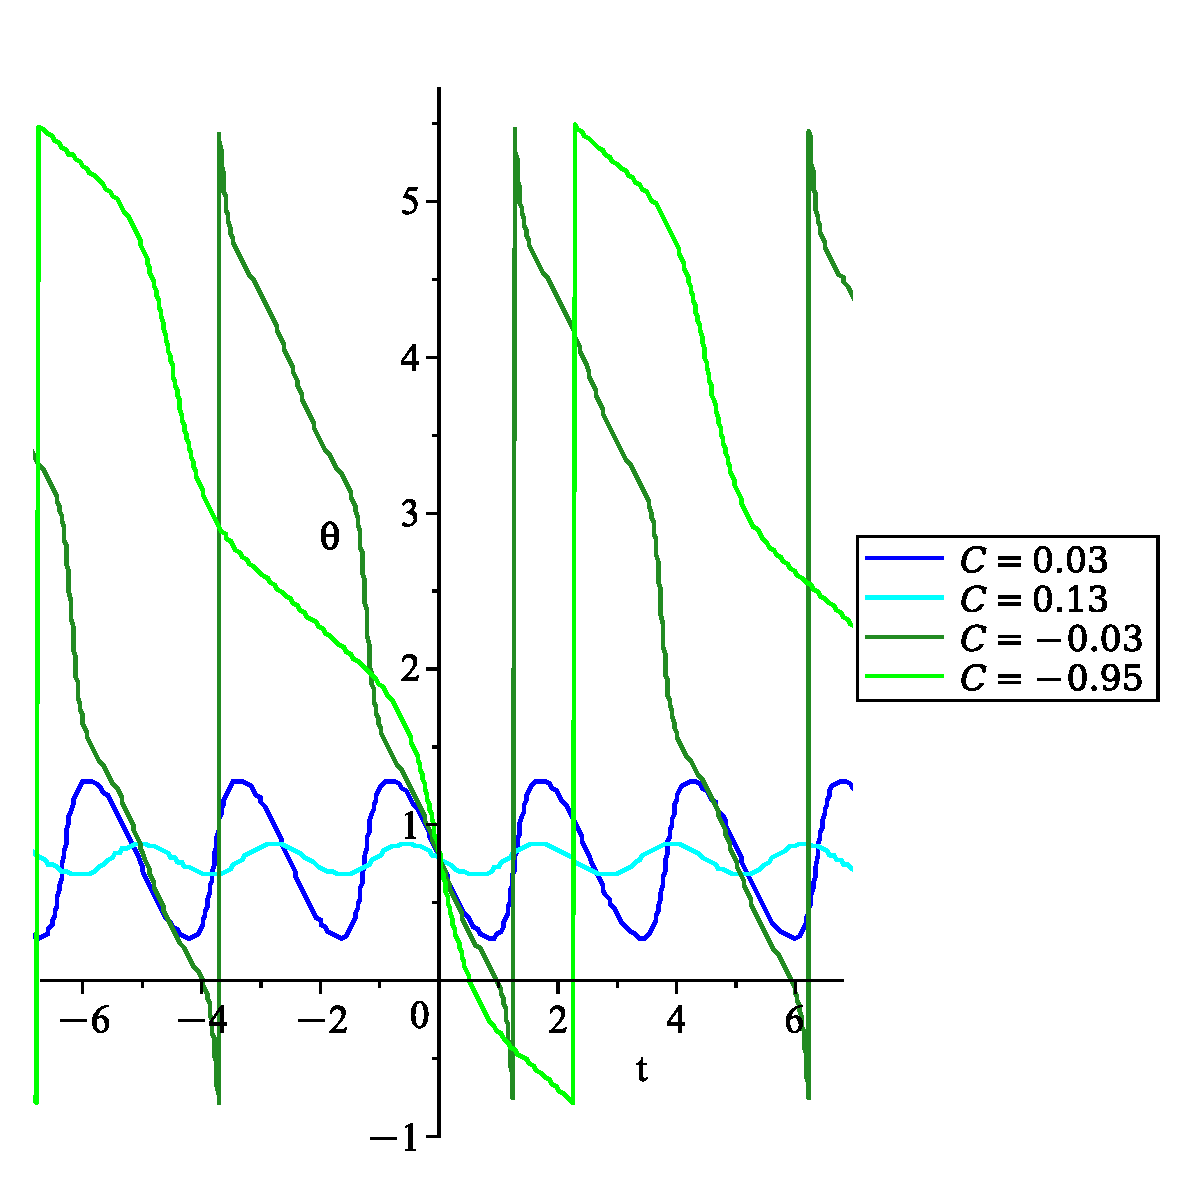
\includegraphics[scale = 0.48]{thetan2.eps}
    \caption{Графики $\Theta_-^\pm(t,0,r_*(C), C)$}%
    \label{fig:eight}
    \end{center}%
\end{figure}

Запишем решение задачи Коши для любых начальных данных $(x_0, y_0, t_{init})$. Тогда $r_{init} = \sqrt{x_0^2 + y_0^2}$, $\theta_0 = \arctan2(y_0, x_0)$(\href{https://en.wikipedia.org/wiki/Atan2}{известная функция}), $C_{0} = (x_0y_0 - 1)e^{(x_0^2+y_0^2)/2}$. Рассмотрим все случаи:
\begin{enumerate}
    \item[{1)}] при $C_0 = 0$ имеем решение $(x(t), y(t)) = (x_0e^{t-t_{init}}, x_0^{-1}e^{-t+t_{init}}),$ $t\in \mathbb{R}$;
    \item[{2)}] при $C_0 = -1$ $(x(t), y(t)) = (0,0),$ $t\in \mathbb{R}$;
    \item[{4)}] при $C_0 = e^{-2}$ имеем два случая. Если $x_ 0> 0$, то $(x(t), y(t)) = (\sqrt{2},\sqrt{2}),$ $t\in \mathbb{R}$. Если $x_ 0< 0$, то $(x(t), y(t)) = (-\sqrt{2},-\sqrt{2}),$ $t\in \mathbb{R}$;
\item[{5)}] при $C_0\in(0,e^{-2})$ имеем четыре случая:\\
если $\theta_0 \in (-\pi/4, \pi/4]$:
$ \begin{cases}
       x(t) = R_+(t,t_{init}, r_{init}, C_0)\cos(\Theta^+_+(t,t_{init},r_{init},C_0)),\\
       y(t) = R_+(t,t_{init}, r_{init}, C_0)\sin(\Theta^+_+(t,t_{init},r_{init},C_0));
\end{cases}$ \\
если $\theta_0 \in (\pi/4, 3\pi/4]$:
$ \begin{cases}
       x(t) = R_-(t,t_{init}, r_{init}, C_0)\cos(\Theta^+_-(t,t_{init},r_{init},C_0)),\\
       y(t) = R_-(t,t_{init}, r_{init}, C_0)\sin(\Theta^+_-(t,t_{init},r_{init},C_0));
\end{cases}$ \\
если $ \theta_0 \in (3\pi/4, \pi)\cup(-\pi, -3\pi/4]$:\\
$\hspace{125pt} \begin{cases}
       x(t) = -R_+(t,t_{init}, r_{init}, C_0)\cos(\Theta^+_+(t,t_{init},r_{init},C_0)),\\
       y(t) = -R_+(t,t_{init}, r_{init}, C_0)\sin(\Theta^+_+(t,t_{init},r_{init},C_0));
\end{cases}$ \\
если $\theta_0 \in (-3\pi/4, -\pi/4]$:\\
$\hspace{125pt} \begin{cases}
       x(t) = -R_-(t,t_{init}, r_{init}, C_0)\cos(\Theta^+_-(t,t_{init},r_{init},C_0)),\\
       y(t) = -R_-(t,t_{init}, r_{init}, C_0)\sin(\Theta^+_-(t,t_{init},r_{init},C_0));
\end{cases}$ \\
\begin{center}
    $t\in \mathbb{R}$
\end{center}

\item[{6)}] аналогично, для $C_0\in(-1,0)$ имеем четыре случая:\\
если $\theta_0 \in (-\pi/4, \pi/4]$:
$ \begin{cases}
       x(t) = R_+(t,t_{init}, r_{init}, C_0)\cos(\Theta^-_+(t,t_{init},r_{init},C_0)),\\
       y(t) = R_+(t,t_{init}, r_{init}, C_0)\sin(\Theta^-_+(t,t_{init},r_{init},C_0));
\end{cases}$ \\
если $\theta_0 \in (\pi/4, 3\pi/4]$:
$ \begin{cases}
       x(t) = R_-(t,t_{init}, r_{init}, C_0)\cos(\Theta^-_-(t,t_{init},r_{init},C_0)),\\
       y(t) = R_-(t,t_{init}, r_{init}, C_0)\sin(\Theta^-_-(t,t_{init},r_{init},C_0));
\end{cases}$ \\
если $ \theta_0 \in (3\pi/4, \pi]\cup(-\pi, -3\pi/4]$:\\
$\hspace{125pt} \begin{cases}
       x(t) = -R_+(t,t_{init}, r_{init}, C_0)\cos(\Theta^-_+(t,t_{init},r_{init},C_0)),\\
       y(t) = -R_+(t,t_{init}, r_{init}, C_0)\sin(\Theta^-_+(t,t_{init},r_{init},C_0));
\end{cases}$ \\
если $\theta_0 \in (-3\pi/4, -\pi/4]$:\\
$\hspace{125pt} \begin{cases}
       x(t) = -R_-(t,t_{init}, r_{init}, C_0)\cos(\Theta^-_-(t,t_{init},r_{init},C_0)),\\
       y(t) = -R_-(t,t_{init}, r_{init}, C_0)\sin(\Theta^-_-(t,t_{init},r_{init},C_0));
\end{cases}$ \\
\begin{center}
    $t\in \mathbb{R}$
\end{center}
\end{enumerate}

Таким образом, мы получили решение задачи Коши для произвольных начальных данных $(x_0, y_0, t_{init})$.\\

После добавления определенного малого возмущения 3-его порядка изначальная система (\ref{eq:first}) примет вид:
\begin{equation}
\begin{cases}
      \dot x=-xy^2+x+y-\epsilon x^3,\\
      \dot y=-x-y+x^2y+\epsilon y^3.
    \end{cases}
    \label{eq:second}
\end{equation}

Для начала составим интегрируемую комбинацию. Используя те же соображения, что и в работе \cite{basov}, получаем два соотношения:
\begin{equation*}
\dot{xy} = (x^2-y^2)(xy(1-\epsilon)-1)\hbox{,\hspace{10pt}} \dot x^2+\dot y^2 = 2(x^2-y^2)(1-\epsilon(x^2+y^2)).
\end{equation*}

Подставляя отсюда $x^2-y^2$ из второго уравнения в первое получаем интегрируемую комбинацию $d(x^2+y^2)2^{-1}(1-\epsilon(x^2+y^2))^{-1}=d(xy)(xy(1-\epsilon)-1)^{-1}$ ,или $xy(1-\epsilon)=1$, или $\epsilon(x^2+y^2)=1$.\\

Интегрируя, получаем первый интеграл системы (\ref{eq:second}) 

\begin{equation}
    (1-\epsilon)^{-1}\ln|(1-\epsilon)xy -1|+2^{-1}\epsilon^{-1}\ln{|\epsilon(x^2+y^2)-1|}=C
\end{equation}

Минуя все вычисления, имеем семь особых точек системы (\ref{eq:second}) при $\epsilon > 0$: $(0,0)$, $(u-v,u+v)$, $(v-u,-u-v)$, $(u+v,u-v)$, $(-u-v,v-u)$,$(\sqrt{2}(1+\epsilon)^{-1/2}, \sqrt{2}(1+\epsilon)^{-1/2})$, $(-\sqrt{2}(1+\epsilon)^{-1/2}, -\sqrt{2}(1+\epsilon)^{-1/2})$, где $u=\cfrac{1}{2}(\epsilon^{-1}+2(1-\epsilon)^{-1})^{1/2}$, $v= \cfrac{1}{2}(\epsilon^{-1}-2(1-\epsilon)^{-1})^{1/2}$.

 \begin{thebibliography}{1}
\bibitem{basov} Басов В.В. \flqq 	Обыкновенные дифференциальные уравнения. Лекции и практические занятия\frqq. 2023, pp. 1223-1235.
\bibitem{engl} Басов В.В. \flqq 	Обыкновенные дифференциальные уравнения. Лекции и практические занятия\frqq. 2023, pp. 1223-1235.
\end{thebibliography}
\end{document}